\documentclass[default]{beamer}
\setbeamertemplate{navigation symbols}{}

\usetheme{CambridgeUS}
\useoutertheme{infolines}
%\usecolortheme{crane}

\usepackage{cmap}							% Поддержка поиска русских слов в PDF (pdflatex)
\usepackage[T2A]{fontenc}       			%поддержка кириллицы
\usepackage[utf8]{inputenc}					% Выбор языка и кодировки
\usepackage[english, russian]{babel}

\graphicspath{{../../images/mpf/}} 			% Пути к изображениям

\makeatletter
\setbeamertemplate{footline}
{
	\leavevmode%
	\hbox{%
		\begin{beamercolorbox}[wd=.333333\paperwidth,ht=2.25ex,dp=1ex,center]{author
				in head/foot}%
			\usebeamerfont{author in
				head/foot}\insertshortauthor~~\beamer@ifempty{\insertshortinstitute}{}{(\insertshortinstitute)}
		\end{beamercolorbox}%
		\begin{beamercolorbox}[wd=.333333\paperwidth,ht=2.25ex,dp=1ex,center]{title in
				head/foot}%
			\usebeamerfont{title in head/foot}\insertshorttitle
		\end{beamercolorbox}%
		\begin{beamercolorbox}[wd=.333333\paperwidth,ht=2.25ex,dp=1ex,right]{date in
				head/foot}%
			\usebeamerfont{date in head/foot}\insertshortdate{}\hspace*{2em}
			\insertframenumber{}\hspace*{2ex} 
		\end{beamercolorbox}
	}%
	\vskip0pt%
}

\setbeamertemplate{bibliography entry title}{}
\setbeamertemplate{bibliography entry location}{}
\setbeamertemplate{bibliography entry year}{}
\setbeamertemplate{bibliography entry note}{}
\bibliographystyle{gost2008p}

\begin{document}
	
	\title[Semiotic schemas]{Знаковые схемы Роя}
	\author[Панов]{Александр Панов}
	\institute[ИСА РАН]{ИСА РАН}
	\date{10 июня 2015~г.} 
	
	\begin{frame}
		\titlepage
	\end{frame}
	
	\begin{frame}
		\frametitle{Деб Рой}
		
		\begin{itemize}
			\item Деб Рой, 43 года "--- специалист по социальным коммуникациям, развитию и нейрофизиологическим основаниям речи.
			\item Профессор Массачутского технологического института, директор \href{http://socialmachines.media.mit.edu/}{лаборатории социальных процессов}, научный консультант в Twitter.
			\item Scopus: 75 статей, 1737 цитирований, h-индекс "--- 16.
			\item Основные публикации:

			{
				\scriptsize
				\nocite{*}
				\bibliography{roy}
			}
		\end{itemize}
	\end{frame}
	
	\begin{frame}
		\frametitle{Цель работы}
		
		\begin{columns}
			\begin{column}{0.7\textwidth}
				\begin{figure}
					\begin{itemize}
						\item Разработка вычислительной модели связи восприятия, моторных действий и семантикой (речевых актов).
						\item Создание целостного (holistic) подхода к определению лингвистического значения.
						\item Решение проблемы оснований символа (symbol grounding problem).
						\item Реализация модели на роботе, способном к выполнению простых действий и простой коммуникации с человеком.
					\end{itemize}
				\end{figure}
			\end{column}
			\begin{column}{0.3\textwidth}
				\begin{figure}
					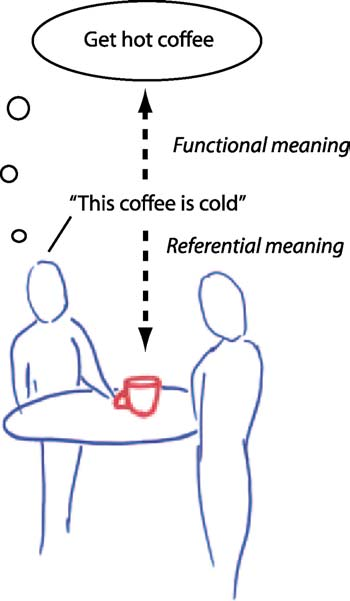
\includegraphics[width=\textwidth]{roy_meaning}
					{
							\scriptsize
							\textit{Референтное vs функциональное значение}
					}
				\end{figure}
			\end{column}
		\end{columns}
		
	\end{frame}	

	\begin{frame}
		\frametitle{Базовые принципы}
		
		\begin{itemize}
			\item Использование \textbf{теории схем} (М.\,А.~Арбиб, Г.~Дрешер, М.~Минский, У.~Найссер, Дж.~Пиаже, Р.~Шэнк) для представления знаний.
			\item Идеи \textbf{семиотики} (Ф.~Дретск, Р.\,Г.~Милликан, К.\,К.~Одген, К.\,С.~Пирс) для определения значения схем.
			\item Статистические \textbf{методы машинного обучения} для реальных систем <<заземлённого языка>>.
			\item Использование \textbf{обратной связи} для генерации устойчивого целенаправленного поведения.
		\end{itemize}
	\end{frame}

	\begin{frame}
		\frametitle{Недостатки символьного подхода}
		
		\begin{itemize}
			\item Многие графы (семантические сети, онтологии и т.~п.), используемые для определения значения, имеют циклы.
			\item Знание, заложенное в робота разработчиком, не является \textit{собственным} знанием робота, что не позволяет ему эффективного решать задачи.
			\item Системы обработки языка, которые опираются только на символьное представление, не имеют встроенных средств фальсификации и проверки.
		\end{itemize}
	\end{frame}

	\begin{frame}
		\frametitle{Вычислительная семиотика Роя}
		
		\begin{center}
			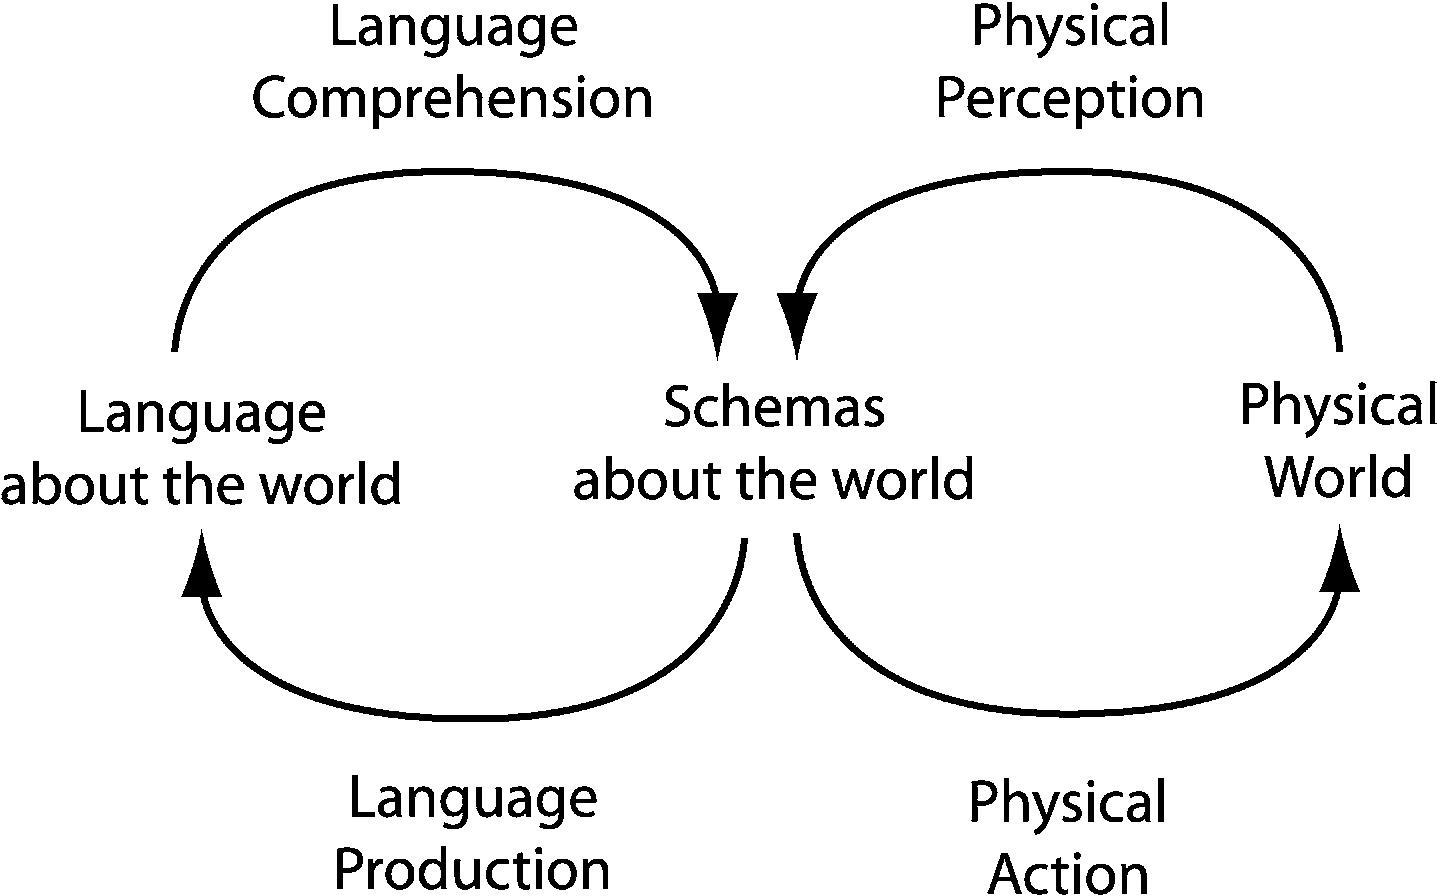
\includegraphics[width=0.4\textwidth]{roy_grounding}
		\end{center}

		\begin{itemize}
			\item Cхемы "--- это информационные структуры, принадлежащие агенту, модифицируемые перцептивными сигналами и направляющие действия агента.
			\item Агент использует схемы для описания своих представлений (beliefs) об окружающем мире.
			\item Процесс обоснования знака (symbol grounding) используется как \textbf{каузальные}, так и \textbf{предсказывающие} отношения между референт и представлением агента.
		\end{itemize}
	\end{frame}

	\begin{frame}
		\frametitle{Принципы вычислительной семиотики}
		
		\begin{itemize}
			\item Описания объектов, свойств, событий и ситуаций строятся с использованием один и тех же примитивов.
			\item Кроссмодальная трансформируемость представлений из восприятия в язык и обратно.
			\item Моторные  и речевые действия должны принадлежать одному пространству действий.
		\end{itemize}
	\end{frame}

	\begin{frame}
		\frametitle{Знаки о отношения на множестве знаков}
		
		\begin{itemize}
			\item Знак понимается в смысле Пирса: имя, референт и представление.
			\item Знак является абстракцией и содержит только значимую информацию о референте.
			\item Знаки классифицируются в три типа: 
			\begin{itemize}
				\item физические (natural) "--- фотоны от летящей птицы,
				\item произвольные (intentional) "--- фраза <<это птица!>>и
				\item индексные (indexical) "--- положение птицы относительно субъекта.
			\end{itemize}
			\item Аналоговые знаки "--- конкретный паттерн, составленный сигналами сенсоров (например, пара значений высоты и ширины объекта "--- это аналоговый знак).		
			\item Аналоговое представление "--- это распределение по всем возможным значениям аналоговых знаков, как история наблюдений и предсказание будущего наблюдения (вероятностная функция на парах высота"--~ширина).
		\end{itemize}
	\end{frame}

	\begin{frame}
		\frametitle{Проекции}
		
		\begin{center}
			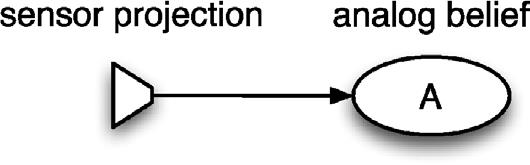
\includegraphics[width=0.3\textwidth]{roy_sens_proj}
			\par\bigskip
			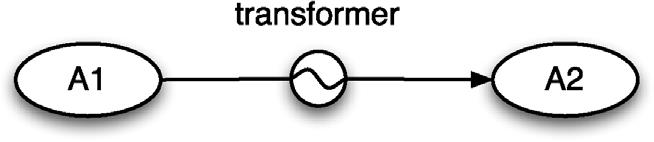
\includegraphics[width=0.4\textwidth]{roy_transf_proj}
		\end{center}
		Представления о дискретных категориях и действия через проекции.
		\begin{center}
			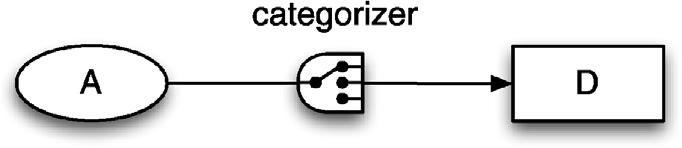
\includegraphics[width=0.4\textwidth]{roy_cat_proj}
		\end{center}
	\end{frame}
	
	\begin{frame}
		\frametitle{Схема действия}
		
		\begin{center}
			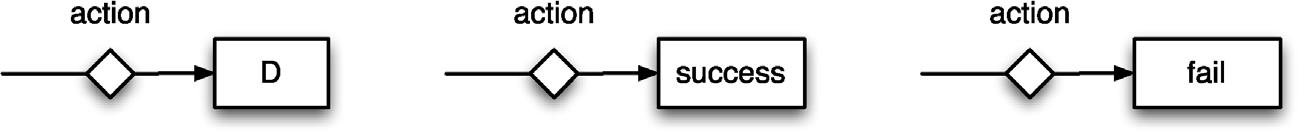
\includegraphics[width=0.8\textwidth]{roy_act_proj}
			\vspace{1cm}			
			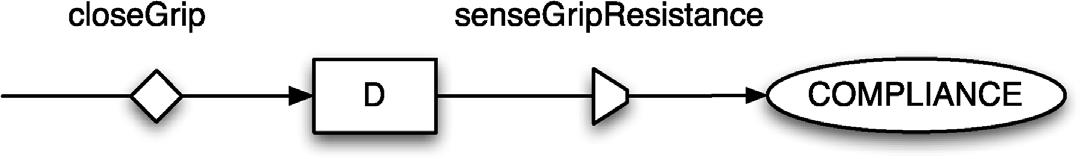
\includegraphics[width=0.7\textwidth]{roy_active}
			\vspace{1cm}
			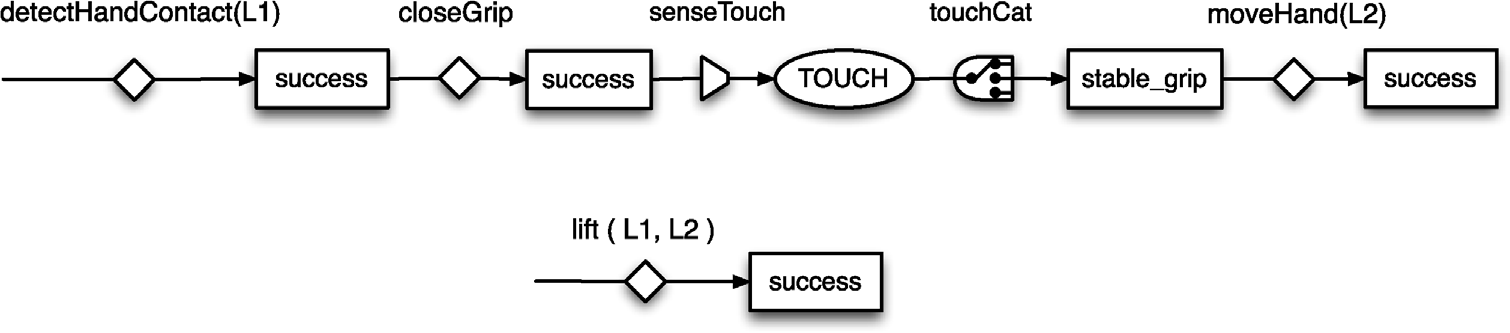
\includegraphics[width=0.9\textwidth]{roy_complex}
		\end{center}
	\end{frame}

	\begin{frame}
		\frametitle{Схема объекта}

		\begin{center}
			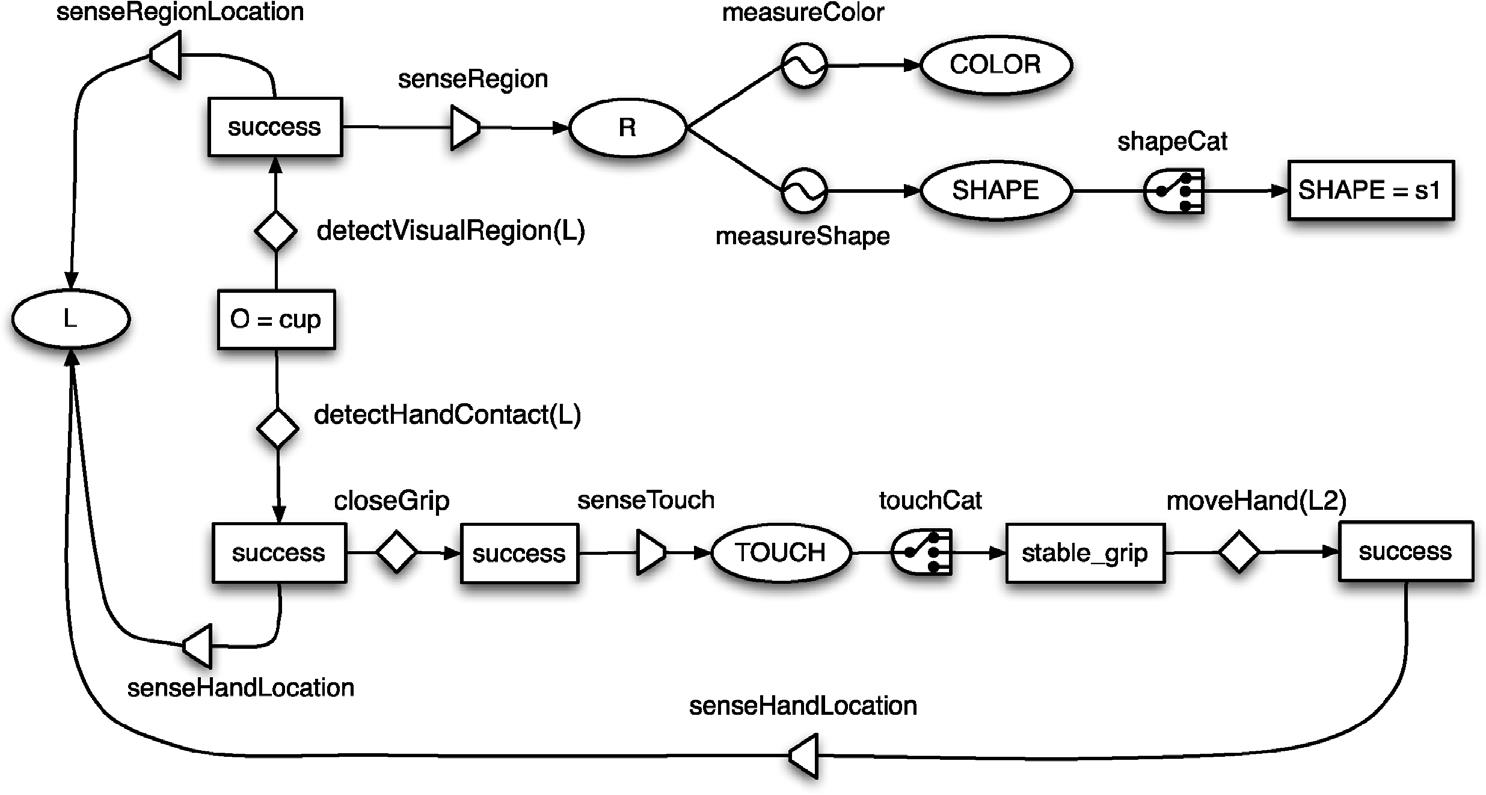
\includegraphics[width=0.9\textwidth]{roy_object}
		\end{center}
		
	\end{frame}
	
	\begin{frame}
		\frametitle{Схема ситуации}

		\begin{center}
			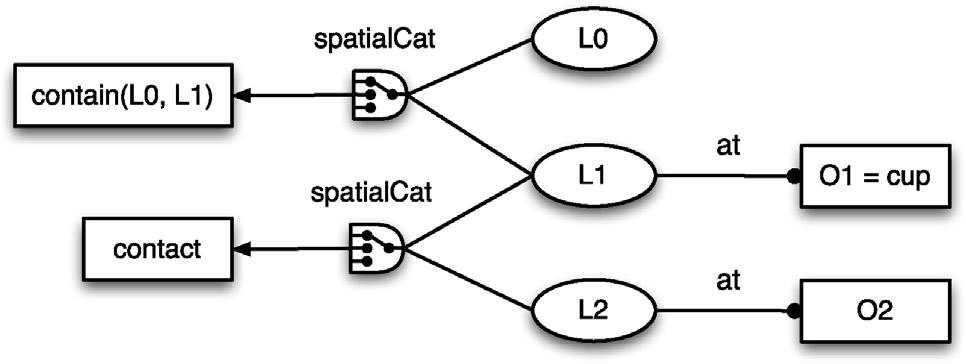
\includegraphics[width=0.4\textwidth]{roy_situation_1}
			\vspace{5mm}
			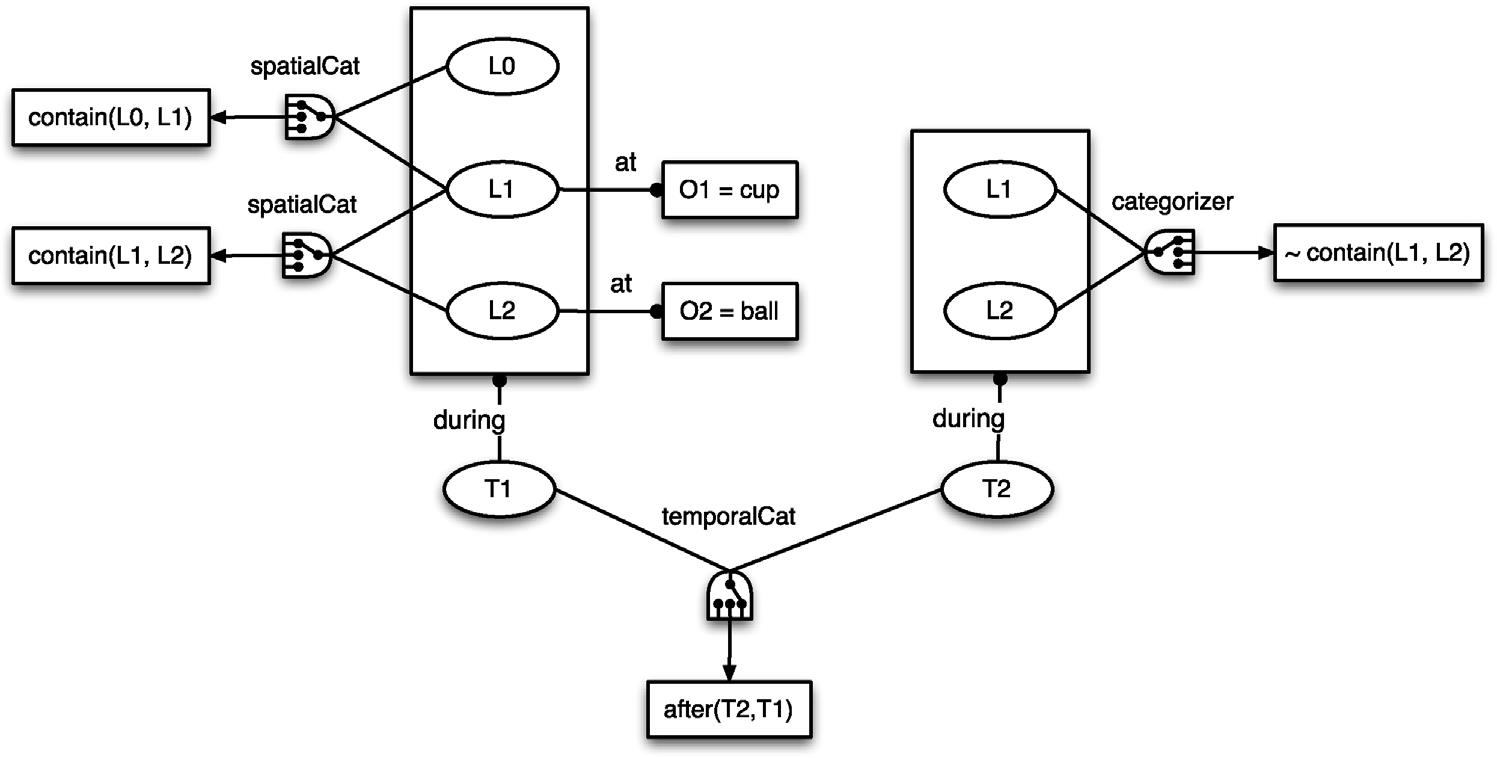
\includegraphics[width=0.8\textwidth]{roy_situation_2}
		\end{center}
	\end{frame}

	\begin{frame}
		\frametitle{Цель и планирование}
		
		\begin{center}
			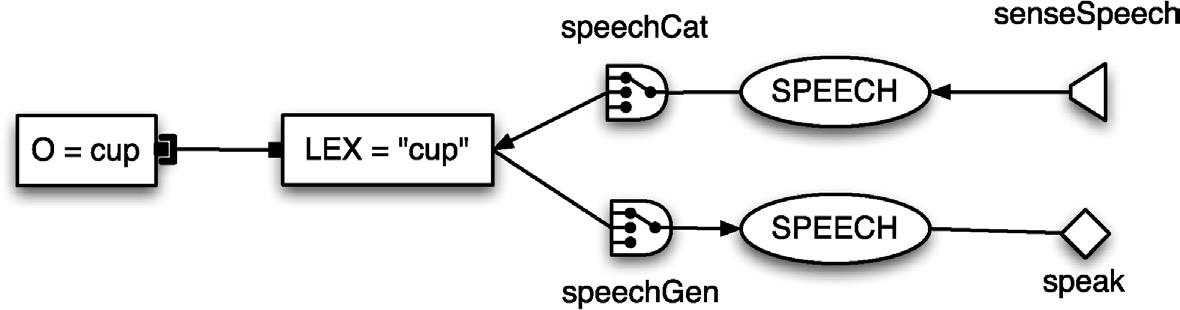
\includegraphics[width=0.8\textwidth]{roy_grounded}
			\vspace{2cm}
			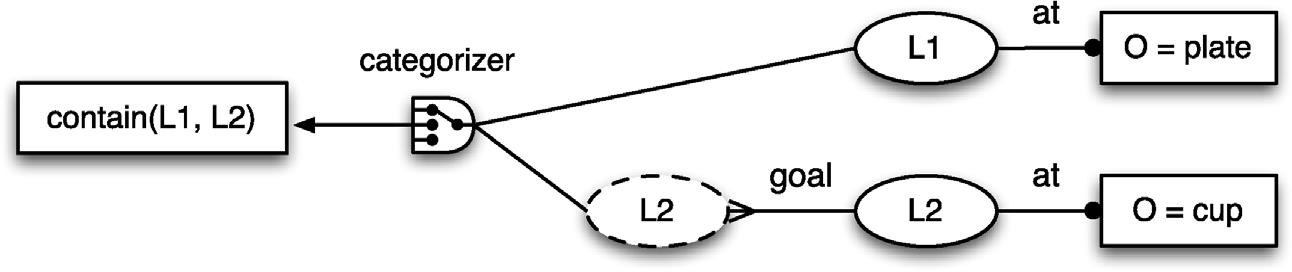
\includegraphics[width=0.8\textwidth]{roy_goal}
		\end{center}
	\end{frame}
			
	\begin{frame}
		\frametitle{Робот Рипли}
		
		\begin{center}
			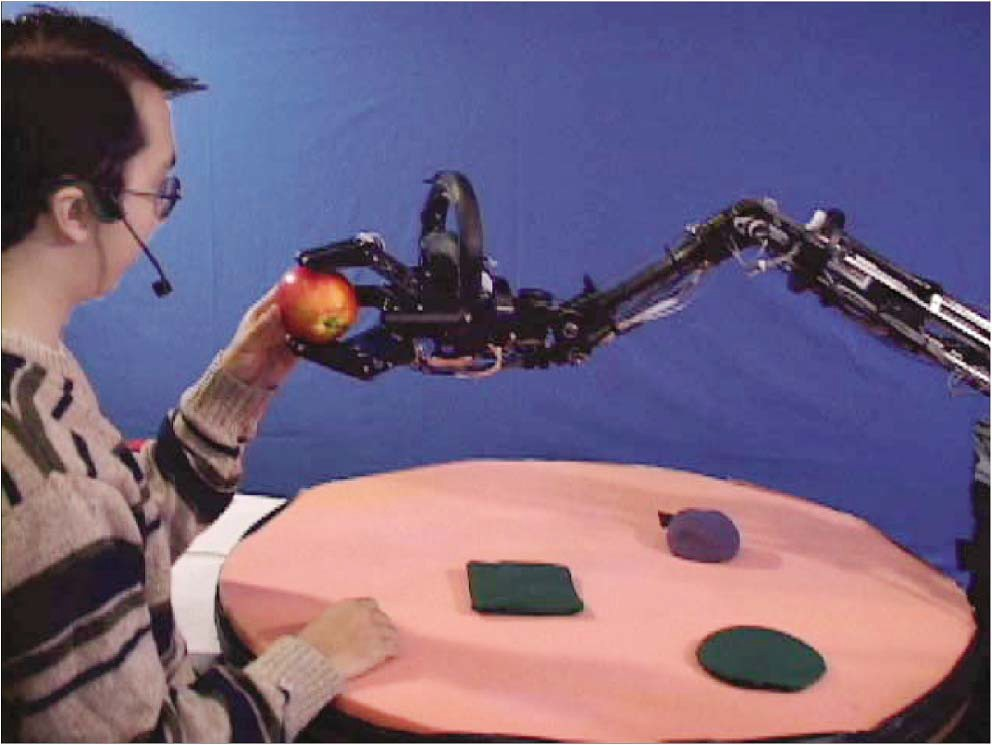
\includegraphics[width=0.6\textwidth]{roy_robot}
		\end{center}
		
		Put the cup on the plate.
		
		Hand me the heavy one.
	\end{frame}

	\begin{frame}
		\frametitle{Социальная сеть и произвольные знаки}
		
		\begin{center}
			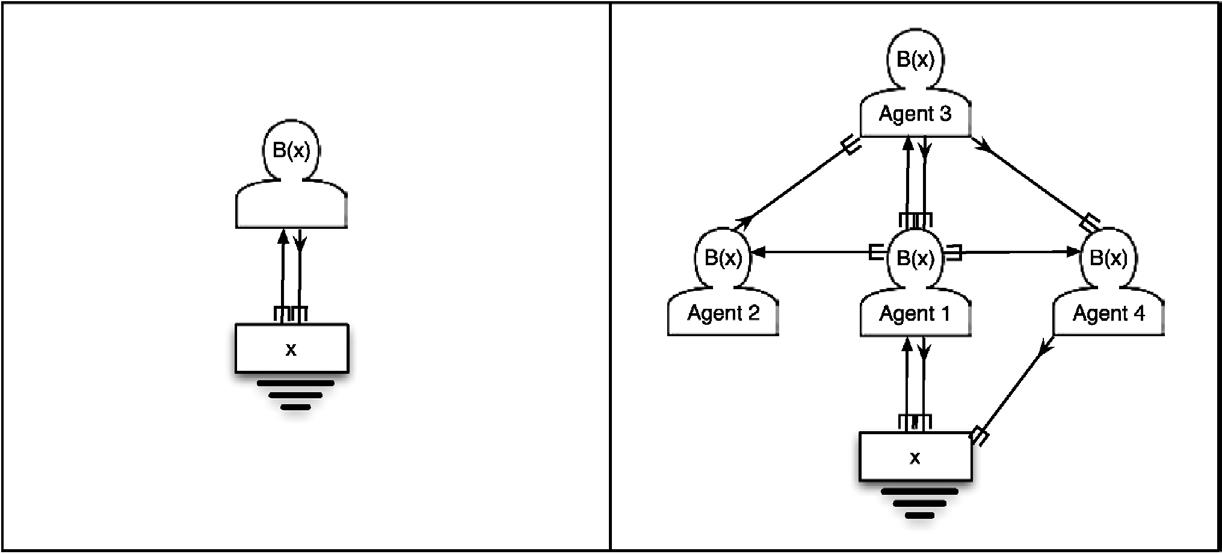
\includegraphics[width=0.9\textwidth]{roy_group}
		\end{center}
	\end{frame}
					
	%	\begin{frame}
	%		\frametitle{Цели курса}
	%		
	%		\begin{itemize}
	%			\item
	%		\end{itemize}
	%	\end{frame}
	
\end{document}
	
	
